\documentclass[11pt]{article}%{IEEEtran}%[conference]{IEEEtran}%\documentclass[10pt]{article}%{article}{report}{letter}{book}{proc}{slides}%
\usepackage{amsmath}
\usepackage{amssymb}
\usepackage{amsthm}
\usepackage{hyperref}
\usepackage{graphicx}
\usepackage{wasysym}
\usepackage{wrapfig}

%\usepackage{skull}

\hypersetup{colorlinks=true,linkcolor=blue,citecolor=blue}

%\textwidth=5.5in
%\oddsidemargin=0.5in
%\evensidemargin=0.0in
%\textheight=8.0in
%\topmargin=0.0in

\begin{document}

\title{Delay Comparison of Different Switch Architectures}



% author names and affiliations
% use a multiple column layout for up to three different
% affiliations
%\author{Stephan Adams and Libin Jiang}
%\IEEEauthorblockA{Department of Electrical Engineering and Computer Science\\
%University of California, Berkeley\\
%\{shadams, jnchang\}@eecs.berkeley.edu}
\author{S. H. Adams, L. Huang, A. Parekh, and J. Walrand }%\author{\IEEEauthorblockN{S. H. Adams, L. Huang, A. Parekh, and J. Walrand \\}}
%\IEEEauthorblockA{Department of Electrical Engineering and Computer Science\\
%University of California, Berkeley\\
%\{shadams,jnchang\}@eecs.berkeley.edu}}


% conference papers do not typically use \thanks and this command
% is locked out in conference mode. If really needed, such as for
% the acknowledgment of grants, issue a \IEEEoverridecommandlockouts
% after \documentclass

% use for special paper notices
%\IEEEspecialpapernotice{(Invited Paper)}

% make the title area


\maketitle

{\abstract
 We compare the delays experienced by packet flows when transmitted using different scheduling algorithms across a crossbar switch.  The two scheduling algorithms we consider are iterative SLIP \cite{McKeown} and QCSMA \cite{Libin}.  We first compare them under the assumptions that all packets have the same length, and then under the assumption that the half the packets have the maximum allowable length and half have the minimum allowable length.  Our findings suggest that the variation in packet length has a non-negligible effect on throughput vs delay results.  For long-lived TCP connections with varying packet lengths, QCSMA derived schedulers seem to do only marginally better than SLIP.  In highly loaded core switches with many short-lived TCP connections, we expect to see a large improvement in delay performance of QCSMA over SLIP.}

\section{Introduction}
Computer networks have made their way to the core of our modern lifestyles.  Almost any information can (and often must) be found on the internet.  Many of the services people use on a daily basis rely on distributed processing of requests housed in enormous datacenters scattered across the country and the world.  All these networks require good routing technologies to be used effectively.

What is the best way to measure the efficacy of a router?  Two obvious metrics are the throughput and delay characteristics of the switches.  Traditionally routers have been evaluated based on their throughput performance.  This is an excellent metric as, in the internet routing, paths are subject to too much uncertainty to hope that optimizing the delays in a single switch to have a large influence on the roundtrip time of your packets.

On the other hand, in a datacenter setting, paths are no longer uncertain, as the whole network is controlled by a single entity.  This allows delay to become a metric worth considering.  The other reason that delay optimization is a metric worth pursuing is because the distributed applications run on datacenters are often very delay sensitive.  User facing applications often ned to return results before a given time threshold or the work must be discarded.%For instance in a google data center any search query must be returned within 300 milliseconds? (CITE SOMEONE) or the work done must be discarded.

Although delay is clearly a very important metric to consider in these settings, it is not as readily analyzed as throughput, which makes it more difficult to give a reliable design recommendation.  In order to model the effects of different switch schedulers we have built a network simulator using assumptions meant to mimic a datacenter environment.  We have compared the performance of two relevant scheduling architectures in the hopes of demonstrating that schedulers that are provably throughput optimal have better delay performance when switches are subjected to high loads.

\section{Switch Schedulers}
We consider two different scheduling algorithms used to route packets across a crossbar based switch.  Iterative SLIP -- a practical scheme design by Nick McKeown to solve the issues of head of line delay \cite{McKeown}, and QCSMA -- a probabilistic scheduling policy developed and optimized to be full throughput by Libin Jiang \cite{Libin}.

Our assumptions on the hardware for both our switches is the same, the only differentiating component is the scheduler which determines which set of packets will be transmitted at each transmission opportunity.  A good scheduler can support an arbitrarily high load, and provides a low delay per packet.  In practice the scheduler will incur some overhead because it takes time to generate a feasible transmission schedule.  The schedulers use an (ideally) small number of contention slots at the beginning of each packet transmission opportunity during which the inputs and the outputs can exchange information to determine the best schedule.  The communication mechanism between the inputs and outputs can be quite powerful in practice.  We assume that each input is connected to each output by a bidirectional one bit line. This allows each output and input to exchange 1 bit in each contention slot.  For the SLIP based scheduler the packets are broken into smaller cells so that the schedules can be generated for a given set of cells, after which they are transmitted over the crossbar, and then the process is repeated.  The QCSMA based algorithms do not synchronize scheduling times, rather it is constantly generating new schedules across the unused portion of the crossbar.

\subsection{SLIP}

Iterative SLIP is a very intuitive and practical scheme invented by Nick Mckeown \cite{McKeown}.  It has been implemented in real systems and yields extremely good performance.  It is difficult to prove anything about this scheduler, but simulations show that it performs very well in many key loading regimes.\\

{\it How it works:}

The motivation behind SLIP was to develop a simple protocol that avoids the use of randomization in the scheduler.  SLIP achieves this by adding a very simple state to the switch.  Each input keeps track of the output to which it last transmitted a packet.  Similarly each output keeps track of the last input from which it received a packet.  Armed with this information, the switch follows these three phases in each contention slot:\\

{\bf SLIP Phases}
\begin{itemize}
\item 1) Every {\it unscheduled} input sends requests to the outputs for which it has at least one packet to deliver.
\item 2) Every {\it unscheduled} output admits the packet request from the input giving round robin priority from the last input it served ($s'$). i.e. first admitting requests from $s'+1$ then $s'+2$ etc.
\item 3) Every input schedules itself for the output that admitted it giving a round robin priority from the last output it transmitted through ($d'$).  i.e. first scheduling an admission from $d'+1$ then $d'+2$ etc.\\
\end{itemize}

After the last contention slot, the scheduled inputs and outputs transmit a single packet and update their state.  Once the packets have been successfully transmitted, the cycle continues.  Note that since the time it takes to transmit a packet depends on its length, there will be a lot of idle time in the system if packet length varies significantly.  In practice this is addressed by breaking packets up into small equal sized cells so scheduling can be done on a cell by cell basis as opposed to a packet by packet basis.  In our simulations we consider both the case of all packets being the same size, and the case in which there is a bimodal distribution of packet sizes.  The overhead necessary to split packets into smaller cells involves adding a header to each cell, and using a larger number of contention slots since they will be needed to schedule per cell size, not packet size.  In our simulations we assumed both of these contributed only a negligible amount to the total delay.

\subsection{Ideal QCSMA}

%Throughput optimal  --> Invented/Explored by Libin and Jean? --> Difficult to Implement

QCSMA is a throughput optimal scheme inspired by Carrier Sense Multiple Access protocols developed for scheduling nodes in a wireless environment.  Because it was designed for wireless environments it assumes a much more restricted feedback model than that used by SLIP, which may be one of the reasons that the practical implementations perform worse than expected.  The only feedback traditional QCSMA assumes to be available takes the form of a broadcast to all inputs or outputs. This differs markedly from the crossbar where it is possible to provide individual feedback to each input and outputs.%, which we will revisit later.

Ideal QCSMA is guaranteed to be full throughput.  Unfortunately the delay performance of flows will depend on the backlog of the queues which they enter, which penalizes low rate flows.  The ideal QCSMA takes place in continuous time: so it can run arbitrarily fast, as well as being immune to collisions, and thus represents a performance bound for the other schedulers.\\

{\it How it works:}

At the beginning of each transmission opportunity, each input $s$ generates an exponential timer $X_{s,d}$ for each nonempty queue  destined for output $d$ (denoted as $Q_{s,d}$).  $X_{s,d}$ is exponentially distributed with rate $\lambda_{s,d} = (Q_{s,d})^{\alpha}$.  Where $\alpha > 0$ is a parameter to be chosen.  Input $s$ then requests access to output $d$ when timer $X_{s,d}$ expires. \\ %There will be no collisions  as this happens in continuous time.\\

{\bf Ideal QCSMA:}
\begin{itemize}
\item {\it unscheduled} input queue $Q_{s,d}$ generates timer value $X_{s,d}\sim \text{exp}(Q_{s,d}^\alpha)$
\item When $X_{s,d}$ expires schedule transmission from input $s$ to output $d$ unless $d$ or $s$ is already scheduled.
\item When a timer expires transmit packets.\\
\end{itemize}

Note the probability of a collision (two or more inputs requesting access to the same output simultaneously) is 0 when the timer values $X_{s,d}$ are continuous.  In simulations we assume that the timer resolution period takes no time, so this scheduling policy can act as an idealized performance benchmark.  This is impossible to implement, so it is necessary to develop a time slotted version that works in a finite number of discrete of contention slots.% although this is unimplementable.  Also note that QCSMA is inspired by Carrier Sense Multiple Access protocols which do not take advantage of the more fine grained feedback available in the switch context, and leveraged by SLIP.

\subsection{Slotted QCSMA} \label{naive_qcsma}

%Approximation of Ideal QCSMA  -->  Hope for similar performance -- Needed to be tweaked to 

In a real system it is not possible to implement continuous time counters, so it is necessary to approximate the continuous time scheduler with a discrete time system.  The scheduling requests for a given output from a given source are made whenever both that output and source are not transmitting any packets and so is not limited to a fixed number of contention slots like that of SLIP.  (We can think of it as in every time slot, performing QCSMA on the portion of the crossbar that is idle.)  Slotted QCSMA approximated exponential timers by geometric random variables determining in which time slot the transmission requests should be made.

If each time slot is assumed to have duration $\beta$, then the probability that an exponential timer of rate $Q_{s,d}^\alpha$ expires within a time slot is given by:
\begin{align}
p'_{s,d} =1-e^{\beta Q_{s,d}^\alpha} \approx \beta Q_{s,d}^\alpha
\end{align}
% in  geometric random variable used to approximate the exponential can approximated by:
We take $p'_{s,d}$ to be the request probability of the input $s$ to output $d$.  When queues get arbitrarily large, the collisions in the system may get excessively frequent (and therefore block transmissions indefinitely), so we limit the aggressiveness of the request rate in order to limit the number of collisions by defining:
\begin{align}  \label{geo_p}
p_{s,d} =\min \left[ \beta Q_{s,d}^\alpha,p_{\text{cap}}\right]
\end{align}

Where we chose $p_{\text{cap}}=.2$.  This then yields the following practical scheme:\\

{\bf Slotted QCSMA:}
\begin{itemize}
\item In the first contention slot for the packet transmission opportunity each input queue calculates $p_{s,d}$
\item {\it unscheduled} input queue $Q_{s,d}$ requests output $d$ with probability $p_{s,d}$.
\item Output $d$ announces the outcome of requests to it.  If there is only one request, $d$ reports success to that input, otherwise $d$ reports collision.%  Upon multiple requests, $d$ reports collision. For no requests, $d$ reports no transmission.
\item If the requests of input $s$ were successful to the outputs in the set $\mathcal{D}$, $s$ schedules itself to output $d$ with probability $\frac{Q_{s,d}}{\sum_{d\in \mathcal{D}}Q_{s,d}}$ (i.e. $s$ chooses among its transmission opportunities in proportion to the queue lengths)
\item Unsuccessful inputs could update $p_{s,d}$ according to one of the schemes below, and re start requesting process\\
\end{itemize}

The performance of this algorithm is expected be quite bad when the packets all have the same length, as it will yield a large number of queues competing for an output at the same time, and therefore also an increased chance of collision.  One possible approach to mitigate this is to adjust the request probabilities using an adaptive sheme. such as the one first proposed by Hajek and van Loon \cite{Hajek_van_Loon}, which was proven to be optimal in wireless environments.  The base probabilities are multiplied by $(1.518,1.000,.559)$  in the event of (no transmission, success, collision).  While this does require a trinary broadcast at the end of each contention slot it is possible to implement the feedback with a binary broadcast as well.  We have shied away from this approach, to compare just the simplest case performance of our different algorithms.



\section{Simulator}

To compare the delay performance of the different schedulers we built an event driven simulator in C++.  Simulation time is discrete with the minimum time step assumed to be the length of one of the bit transmissions of one of the schedulers.   The packet lengths are given in lengths of these time steps.  Because modern crossbars transmit packets in parallel we assume that it takes 5 clock ticks to transmit a 64 byte packet, and 120 clock ticks to transmit a 1500 byte packet.  For all the SLIP simulations we assumed there were $6$ contention slots used to generate the crossbar schedules, but that these calculations were pipelined in such a way as to make the net scheduling negligible compared to the packet transmission time.  Simulation inputs were flow patterns passing through the switch, which were identical for all switches.  We chose to simulate a switch with 32 inputs and 32 outputs as it models a realistically sized switch, which would not take inordinant amounts of time to simulate.%The switch operation was simulated for $10^6$ time steps, in order to reach the steady state switch behavior%during a given experiment in order to avoid  make the comparison between different scheduling policies and module types without worrying about inconsistencies in flow statistics.   

 The simulations fall into two categories: an open loop version meant to measure switch throughput, and a closed loop version meant to mimic TCP operation over the switch.  
 \subsection{Modeling Challenges}
 We encountered several technical challenges that guided our design decisions.%to accurately and efficiently simulate the functioning of a switch.  
 We chose the event driven paradigm to address the modeling limitations of an earlier time driven simulator.  The time driven simulator allowed for a simple calculation of state evolution, but required a tradeoff between efficiency of the simulation and accuracy of our model.  A time driven simulator updates the state by iterating over time steps representing some duration of real time.  The major limitation of this model is that the smallest time between any two state changes is limited by the duration represented by a time step.  Choosing to have each time step represent the smallest relevant time interval in the system is problematic, since the switches we are modeling function on two vastly different time scales: that of contention slots and that of packet transmission times.  Because packet transmissions last significantly longer than contention slots, after a crossbar schedule has been generated there are long stretches of time in which no meaningful changes in state occur.  During this time the simulation would be needlessly recalculating the system's state at every time step.
 
 To avoid this wasted computation, we initially approximated the behavior of the schedulers and assumed that all packets had a uniform length.  We quickly realized that this was not capturing the significant effects we were modeling, and so decided to use an event driven simulation.  Instead of iterating over time, each iteration in an event driven simulator calculates the next event (change in system state) and the time at which it will occur.  This allows us to keep the number of iterations proportional to the number of events  without sacrificing the accuracy of our model.  The main difficulty with this design choice is that the calculation of the next event can be quite complex.
 
Usually the bookkeeping in event driven simulation uses an event queue which stores all generated events that have yet to be applied to the system state.  This can be difficult to implement if an event added to the queue could modify the events already in the queue (e.g. arrivals to the switch would affect the next scheduled transmission).  To avoid these issues, we only kept track of the next event.  We assumed that all random events were geometrically distributed (and thereby memoryless) as a function of the current state.  All the deterministic events could be recalculated from the state resulting after the application of the next event.  This greatly simplified the bookkeeping.

One unforeseen consequence of this approach is that only keeping the next event discarded any concurrent events.  (Concurrent events occur with nonzero probability since the system we are simulating operates in discrete time.)  This was remedied by creating a function to merge two events, which either discarded the later of the two events or created an event that included both state updates if the two events coincided.  This change was extremely important as it significantly changed the outputs of the simulator.

\subsection{Organizational Challenges}
In addition to modeling challenges, there were some organizational challenges to ensuring the simulator would be versatile and easy to use.  

We tried to enforce a modular structure on the different functions used by the simulator.  A key to successfully doing this was the definition of the Event class.  The state of the simulator could only be modified by a well defined Event object.  Event objects then provided a common interface for all functions that simulated components switch.  Every existing component modeled by the simulator takes as an input the current state and outputs an Event object.  New components can be easily added by creating a function that outputs an appropriate Event given the simulators current state.  This is an especially apt abstraction, because the Event class contains the merge function, which allows any two Event objects to be combined in such a way as to produce a single valid Event that incorporates the necessary state updates.  Additional functionality can be easily added to the modeled switch by creating the appropriate functions and merging them with the most recently calculated event.

In addition to trying to modularize all the components of the simulator and giving functions a common interface, there were some organizational functions that made modifying simulation scenarios and generating new sets of data easier.  One was the creation of a single format for recording all the data: the Data\_Collector class.  Collecting new statistics of different kinds was greatly simplified as the Data\_Collection class has a standardized interface for adding data and does all the difficult storage bookkeeping (i.e. creating new arrays and maintaining them).  The other huge advantage of creating this class is that it is outfitted with a function that aggregates and writes all the collected data to an output file with a standardized format.  This greatly decreased the overhead of adjusting which statistics should be collected and adjusting what is written to the output files.

We created three extremely functions designed to easily set up and run simulation scenarios.  The function init\_sim() sets up the initial parameters, the function reset\_sim() reset the state to the appropriate initial conditions, and the function run\_sim() progress the system state through a specified number events.  To run a new simulation it is then only necessary to call these three functions, which allows for extremely simple semantics to run a series of simulations.

As any giant coding project, there were a lot of bugs that had to be tracked down.  The use of a log which wrote error messages to a file rather than generating print statements was quite useful as it was possible to look into the operation of loops without having an unmanageable dump to the terminal.

The choice of simulator language was based on a tradeoff between the desired performance and the ease of writing the code.  The main simulation loop was written in C++ as it is very efficient at performing a large number of loop iterations.  Once the data is generated, efficiency is not as great a concern, so we can feed the data into a Matlab script, since the graphics tools are good and simple to use. 
 
 For more specific details on the simulator design please see appendix \ref{code_design}.%We go into more depth in subsequent sections.
 
\section{Open Loop Simulations} \label{open}

We explored the capacity of the different schedulers by injecting a stream of packets at a given rate into the switch.  For the QCSMA algorithms we also had to do a search for good parameters, and settled on the values in table \ref{qcsma_parameters}.  Once the appropriate parameters had been chosen we generated figures \ref{one_size} and \ref{variable_size} by performing multiple simulations by increasing the fraction $f$ of switch capacity from $.1$ to $.95$.  The load was generated by having flows from every input $s$ to every output $d$.  In each time step, each flow received a new packet with an i.i.d. probability $p=f/32$.

\begin{table}[ht] \caption{QCSMA Parameters} 
\centering 
\begin{tabular}{c c c}
 \hline\hline 
 Algorithm & $\beta$ & $\alpha$ \\
  [0.5ex] \hline 
   QCSMA&.2&.9  \\
   ideal  QCSMA&-&1  \\
   %DCSMA&?&?  \\
  [1ex] \hline 
  \end{tabular}
   \label{qcsma_parameters} 
\end{table}

In figure \ref{one_size}, all the packets were generated to have one size.  In this scenario SLIP performs very well, on par with ideal QCSMA.  Slotted QCSMA incurs the largest delays.

In order to test whether this poor performance was due to the higher collision rate caused by all the packet transmissions beginning and ending almost simultaneously, we performed a second experiment in which we had a bimodal packet distribution over packet lengths.  In this alternate scenario (depicted in figure \ref{variable_size}) we generated packets with an iid probability of being the maximum size (1500 bytes) with probability $1/2$ and the minimum size (64 bytes) with probability $1/2$.  The rationale behind this distribution was to observe that data packets in TCP flows are generally transferring chunks of some larger file (so may as well send the maximum bytes).  For every data packet which makes it through the system, there is a control message, such as an ACK that do not need to be very large so can be modeled as being the minimum data packets.  As shown in figure \ref{variable_size} all the schedulers perform comparably until we reach higher loads.  Above loads of $60\%$ the switch capacity, SLIP starts to perform considerably worse than slotted QCSMA.  Interestingly the performance of the slotted QCSMA follows the performance of the ideal version more closely than in the single packet length scenario.

\begin{figure}
\center
	 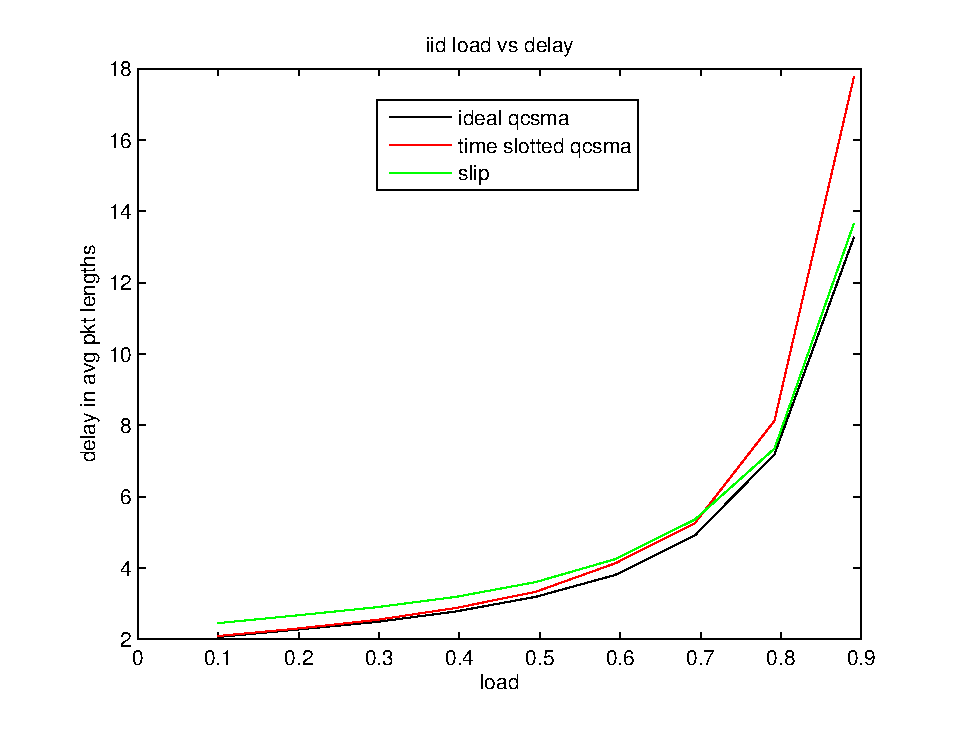
\includegraphics[width=90mm]{us_load.eps}
	\caption{Delay vs throughput graphs for loads in a scenario in which all packet have the same length.  SLIP performs comparably to the ideal QCSMA scheduler, and outperforms the realistic implementation of QCSMA.  The parameters for the QCSMA based schedulers are taken from table \ref{qcsma_parameters}.} 	
	\label{one_size}
\end{figure}

\begin{figure}
\center
	 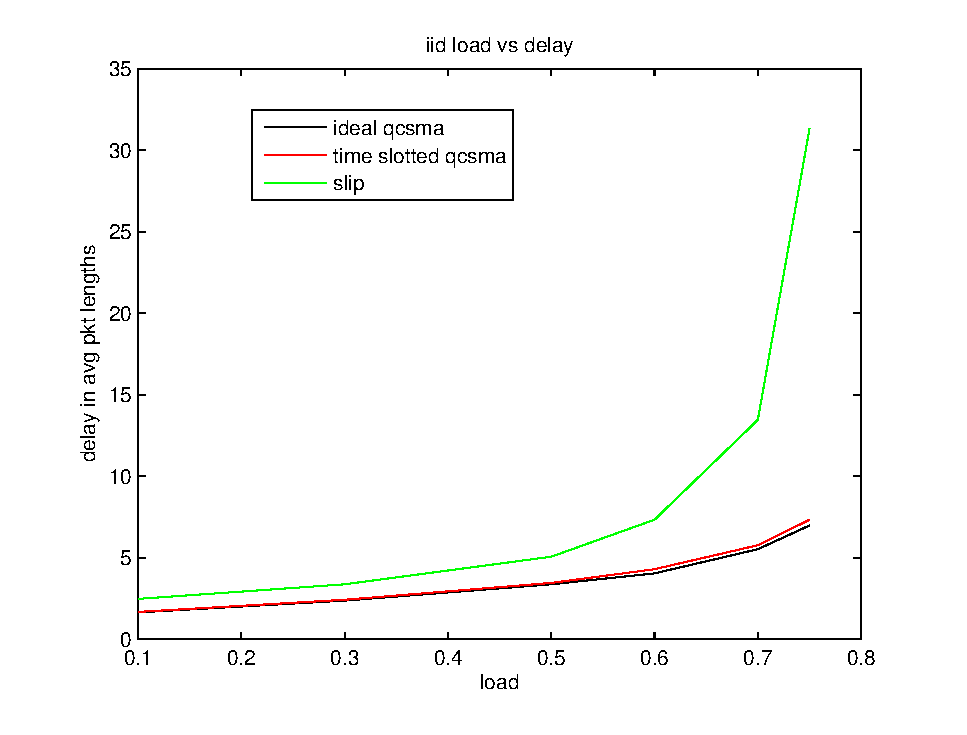
\includegraphics[width=90mm]{vs_load.eps}
	 \caption{Delay vs throughput graphs for loads in a scenario in which every packet has a probability of $1/2$ of being the minimum size and $1/2$ of being the maximum size. With the variable sized packets SLIP no longer outperforms the practical version of QCSMA.  QCSMA still performs similarly to the single length scenario.  (Note that the x axis in this graph is different from that in figure \ref{one_size}.) The parameters for the QCSMA based schedulers are taken from table \ref{qcsma_parameters}.} 	
	\label{variable_size}
\end{figure}

\section{Closed Loop (TCP) Simulations} \label{closed}


Switches are not generally subjected to an unmodulated stream of packet flows.  Rather, the flows between applications are generally regulated via TCP or some other congestion/flow control mechanism.  This results in a different environment under which the differences highlighted by the open loop simulations might only play a negligible role.  To explore this idea, we have added a layer to our simulator which models TCP.  The only difference between our version of TCP and the traditional TCP is that we use Explicit Congestion Notification instead of packet dropping to respond to congestion.  Aside from simplifying the structure of the simulator, this choice reduces the long timeout delays, (or the need to fine tune the estimate of the roundtrip time to avoid this), which result whenever the routers buffers become overwhelmed.  The ECN bit is set with probability $p_{\text{ecn}}$ if the switch queues exceed some threshold $T_{\text{ecn}}$.  The TCP window is then reduced after it receives an ACK with the ECN bit set.  This is only one of the many proposed changes to adapt TCP to a datacenter setting.

We performed a variety of experiments meant to simulate different application communication patterns in datacenters.

As the throughput supported by the different switches seems comparable, we focus on the delay performance of the switches under TCP connections.  TCP Inputs to the simulator can be represented as a flow type matrix such as the one visualized in figure \ref{typical_flows}.  The entry $s,d$ represents the type of flow from input $s$ to output $d$.  We consider two main types of flows, high throughput flows that are relatively insensitive to delay (type 1 flows) and low throughput flows that are sensitive to delays (type 2 flows).  The packets generated for TCP are generated according to Markov ON OFF processes much as in the open loop simulations with one producing a very low throughput set of packets and the other being generating a much higher throughput, in order to simulate the different types of datacenter flows.  The type 1 process has transitions from ON to OFF transition with probability $.3$ and from OFF to ON with probability $.7$.  The type 2 process transitions from ON to OFF with probability $0.0781$ and from OFF to ON with probability $0.9219$.  When the process is ON it generates packets, and it does not when it is OFF.   State transitions occur at each time step.

The TCP window size is updated by additive increase multiplicative decrease, with feedback coming in the form of acks that are generated whenever a packet successfully traverses the switch.  The acks in our simulation are not actually packets sent through our network, but rather simply notify our TCP simulator after an artificially determined delay.  After an ack notifies the TCP flow it adjusts its send window statistics accordingly.  The ack is delayed by a factor of 10 times the delay it took the packet to traverse the switch in order to simulate the round trip time in a datacenter that has five switches between the input and its intended output.

\subsection{Parameter Search}

%In our model there is no maximum buffer size, and consequently no dropped packets.  Consequently, we need to give TCP feedback on when to halve its window size by another means.  We do this by using the explicit congestion control bit in the tcp header.  Our simulations mark packets as facing congestion with a probability $p_{\text{ecn}}$ if the packets arrive at a queue at or exceeding a threshold $T_{\text{ecn}}$ packets.  After our TCP receives an ack which announces that it faced congestion, it will halve it's window, and wait one round trip time before rehalving it's window, in order to flush out all the duplicate congestion announcements due to packets sent before the congestion announcement was received.

  TCP should be optimized for its environment so we conducted a parameter search to determine good values for each of the switches.  While the QCSMA was tuned to perform well for a worst case scenario, for TCP we are interested in improving average performance.  The search for the two parameters $p_{\text{ecn}}$ and $T_{\text{ecn}}$ is conducted over what we consider an average set of average flow statistics for a datacenter, as suggested in \cite{Benson} and \cite{Kandula} and shown in figure \ref{typical_flows}.

%As we assume the new datacenters will be built with a single scheduler in mind, so we search for good TCP parameters for each switch alternative.  
Please see table \ref{ecn_table} for the choices we settled on.  Once we settled on the parameters for TCP we can compare how the different architectures compare with each other for a variety of trial flows.  
%See the figures \ref{tcp_perf}.


We present 4 simulations in which we simulated different flow patterns to our schedulers and observed the average delay per flow.  The flow patterns we investigated were:

\begin{itemize}
\item all to all 
\item spread and aggregate 
%\item three simultaneous spread and aggregate
\item typical 
\item typical and spread and aggregate
\end{itemize}

\subsubsection{All to all (core switch)}
An all to all pattern can be seen in figure \ref{all_to_all_flows}.  The type of each flow (from $s$ to $d$) was drawn from an iid distribution that yielded type 1 with probability $1/2$ and type 2 with probability $1/2$.  This flow pattern was meant to mimic a possible load on a core switch, which has to aggregate the traffic from across the network.  Results suggest that the performance of the switches was very similar.  The throughput for all the switches is about the same, and in terms of delay the difference is not significant. Ideal QCSMA performs mildly better than the other switches.  See figure \ref{all_to_all} for a comparison.

Notably the gain of the unimplementable ideal QCSMA performs by far the best.  Time slotted QCSMA in this scenario also outperforms SLIP, having both a lower average, and lower extremes than SLIP.  While this does match our intuition that the throughput optimal scheme should perform better, it is not nearly as spectacular a result as our open loop simulations would have lead us to expect.


\begin{table}[ht] \caption{TCP Parameters} 
\centering
\begin{tabular}{c c c}
 \hline\hline 
 Switch & $T_{\text{ecn}}$ & $p_{\text{ecn}}$ \\
  [0.5ex] \hline 
 SLIP&10&.5 \\
  QCSMA&12&.5  \\
   ideal  QCSMA&10&.9  \\
  [1.0ex] \hline 
  \end{tabular}
   \label{ecn_table} 
\end{table}


\subsubsection{Spread and Aggregate (MapReduce)}
One of the most famous (if not most popular) applications in modern datacenters is certainly MapReduce.  The communication pattern of MapReduce often involves a large transfer of data to and from a single node between the different phases of computation.  In order to mimic this type of operation we developed a spread and aggregate flow pattern in which a given server sends data to all other servers using high throughput delay insensitve flows (type 1), since the volume of data exchanged between the master and worker servers is often quite large.  An example in which the source of the pattern is on input 1 is shown in figure \ref{spreadagg}
 %low throughput highly delay sensitive flows (type 2), which in turn are returned to the server.   An example in which the source of the pattern is on input 1 is shown in figure \ref{spreadagg}

This does not accurately model a MapReduce job for several reasons.  The biggest departure from a typical MapReduce job is that our type 1 flows do not have similar synchronization or burstiness properties due to the similar completion times of computations in a real MapReduce job.  Furthermore the large delays imposed by the artificial 10 hop distance for the acks is responsible for another difference in our model.  Still we hope that it suffices to give an impression of how a spread and aggregate application might behave.

The performance for the different schedulers can be seen in figure \ref{vs_spreadagg}.  Interestingly, in this scenario the worst performing flow of SLIP does much better than the extreme flows of both the QCSMA schedulers.  Despite this higher variation, both QCSMA schedulers perform better on average than the SLIP scheduler.  The performance difference is not significant in the case of the practical time slotted QCSMA, while the ideal implementation of QCSMA does about 4 times better.  Depending on how close the practical QCSMA implementations can be pushed towards the ideal scheduler, this might be significant.

\begin{figure}
\center
	 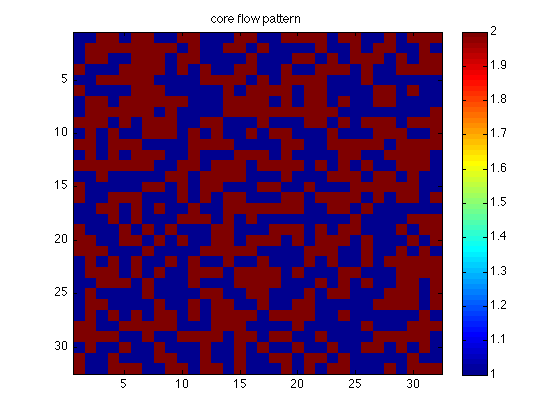
\includegraphics[width=90mm]{all2allflows.png}
	\caption{This graph shows the flows experienced by a core router with all to all traffic the red flows are type 2 while the blue flows are type 1.}
	\label{all_to_all_flows}
\end{figure}

\begin{figure}
\center
	 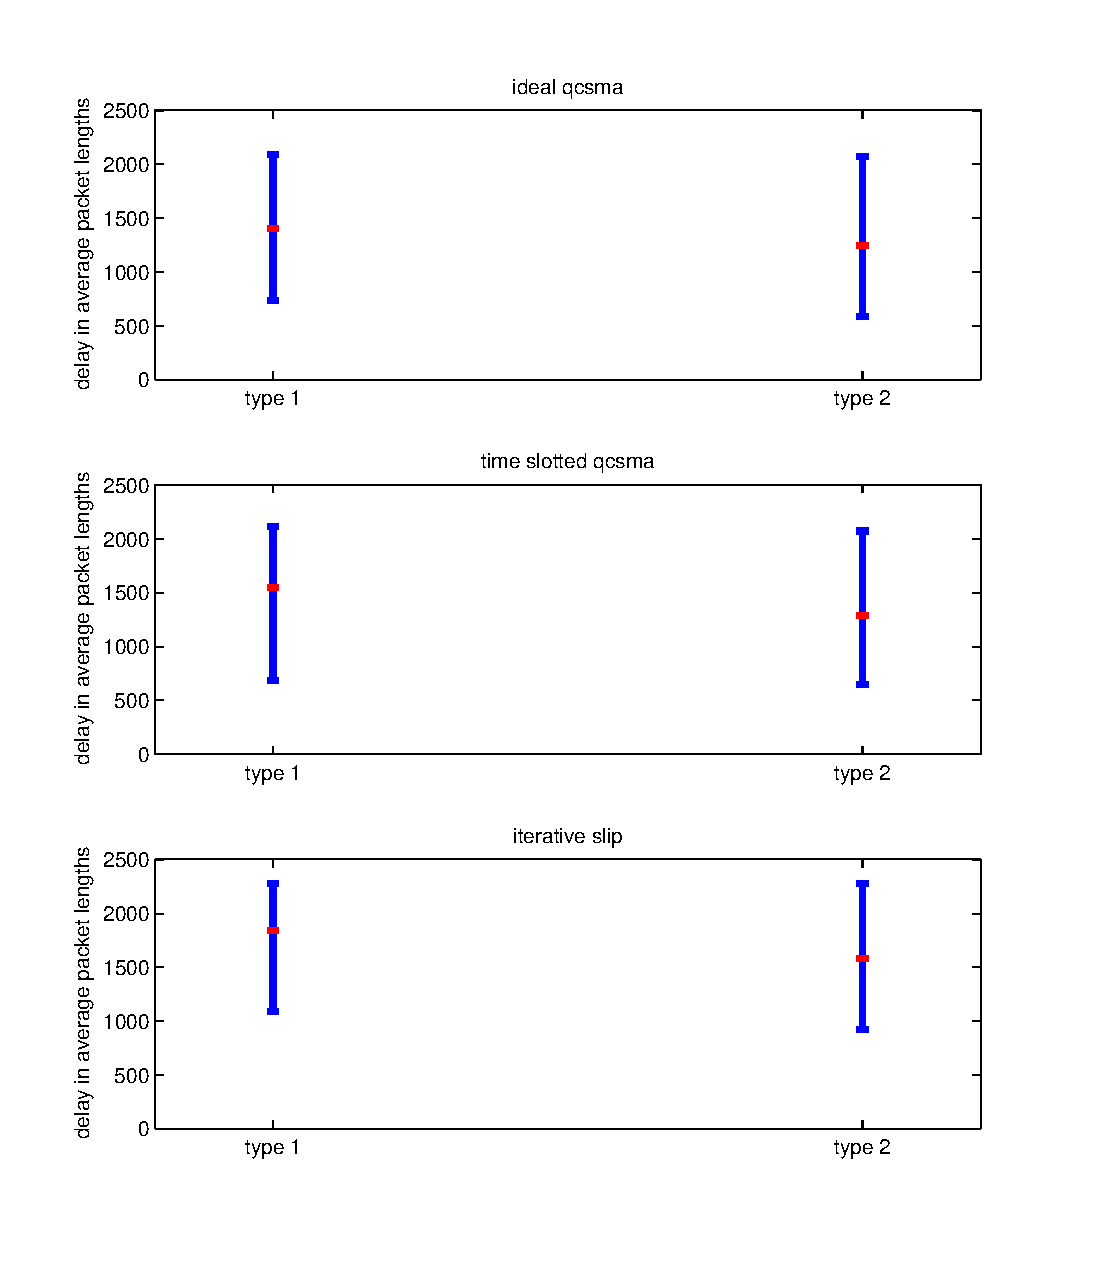
\includegraphics[width=\textwidth]{all_2_all.eps}
	\caption{This graph shows the delays experienced by a core router with all to all traffic.}
	\label{all_to_all}
\end{figure}


\begin{figure}
\center
	 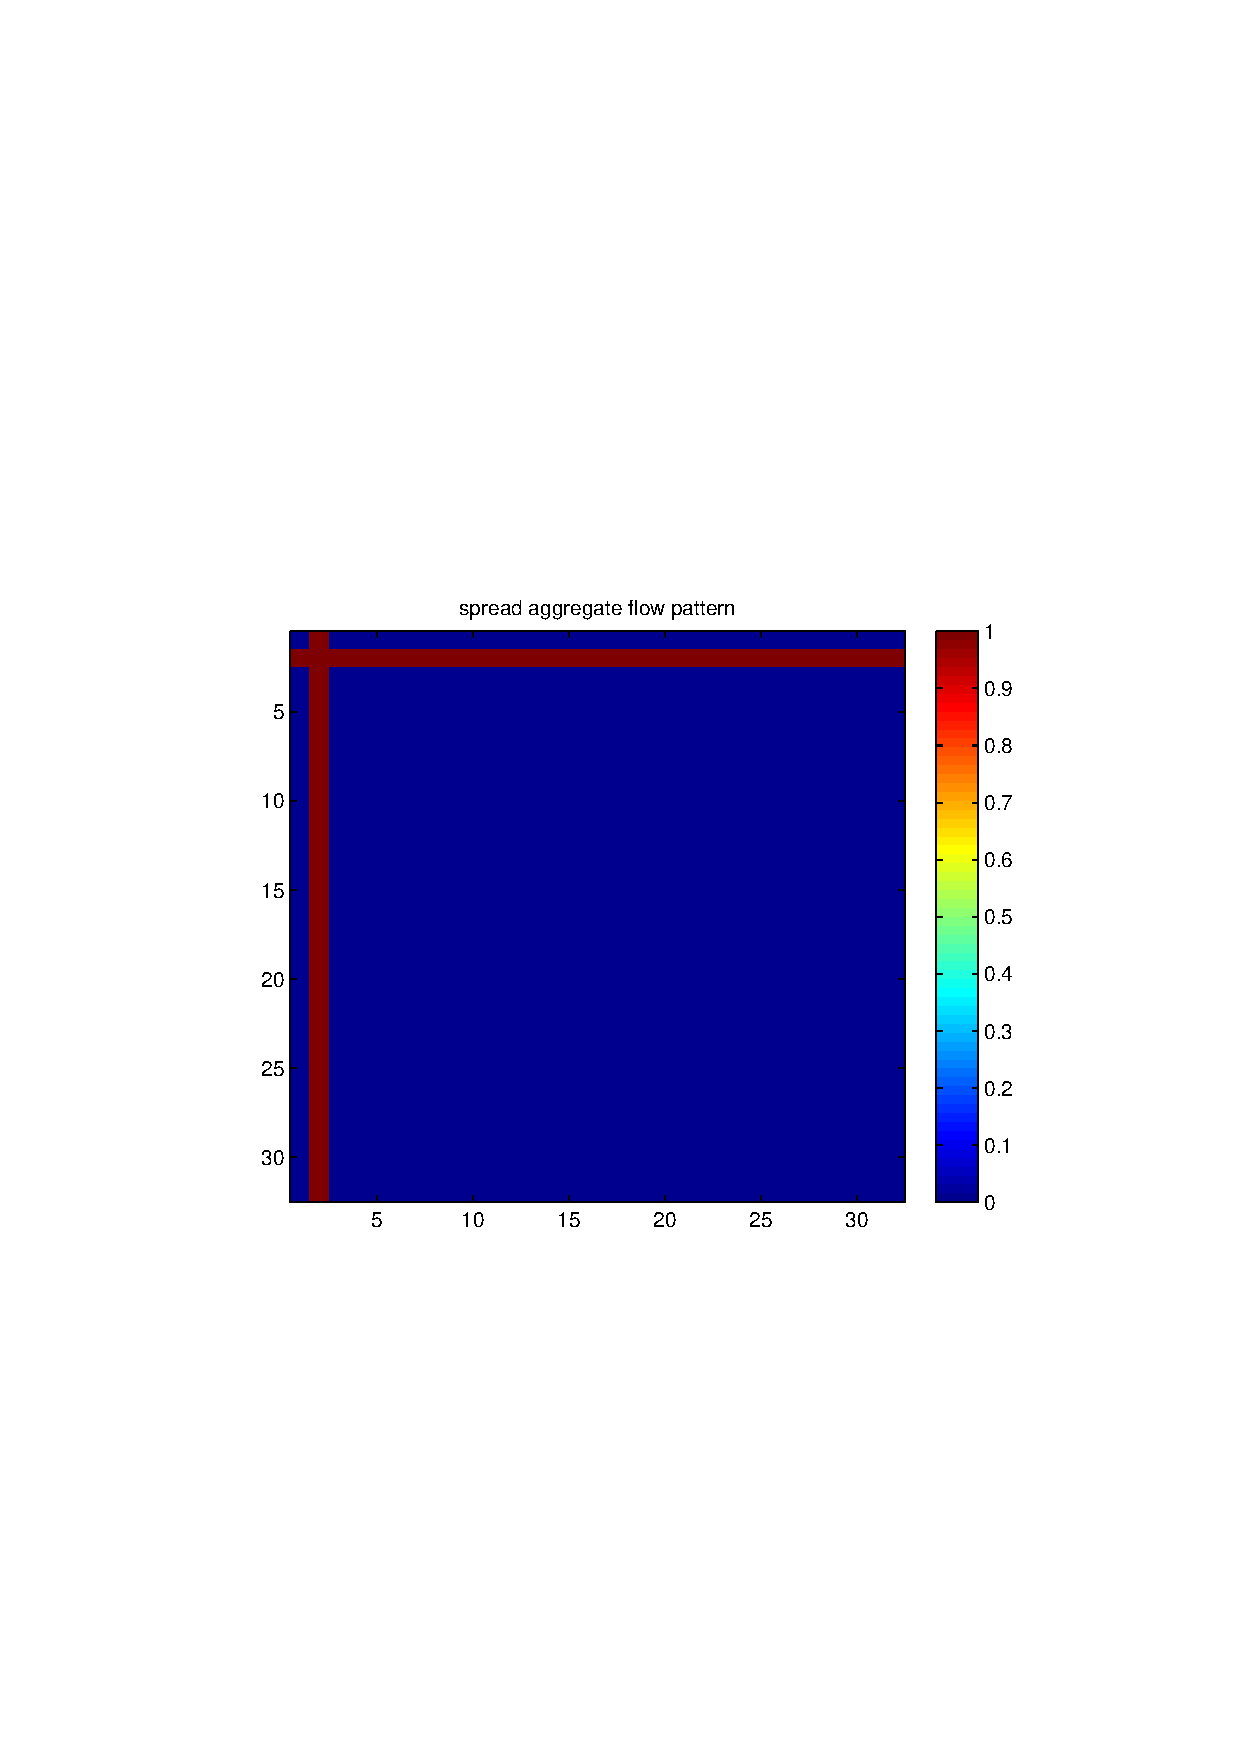
\includegraphics[width=90mm]{spread.png}
	\caption{This graph shows a typical spread aggregate pattern.  In this case the blue flows indicate the absence of a flow..}
	\label{spreadagg}
\end{figure}


\begin{figure}
\center
	 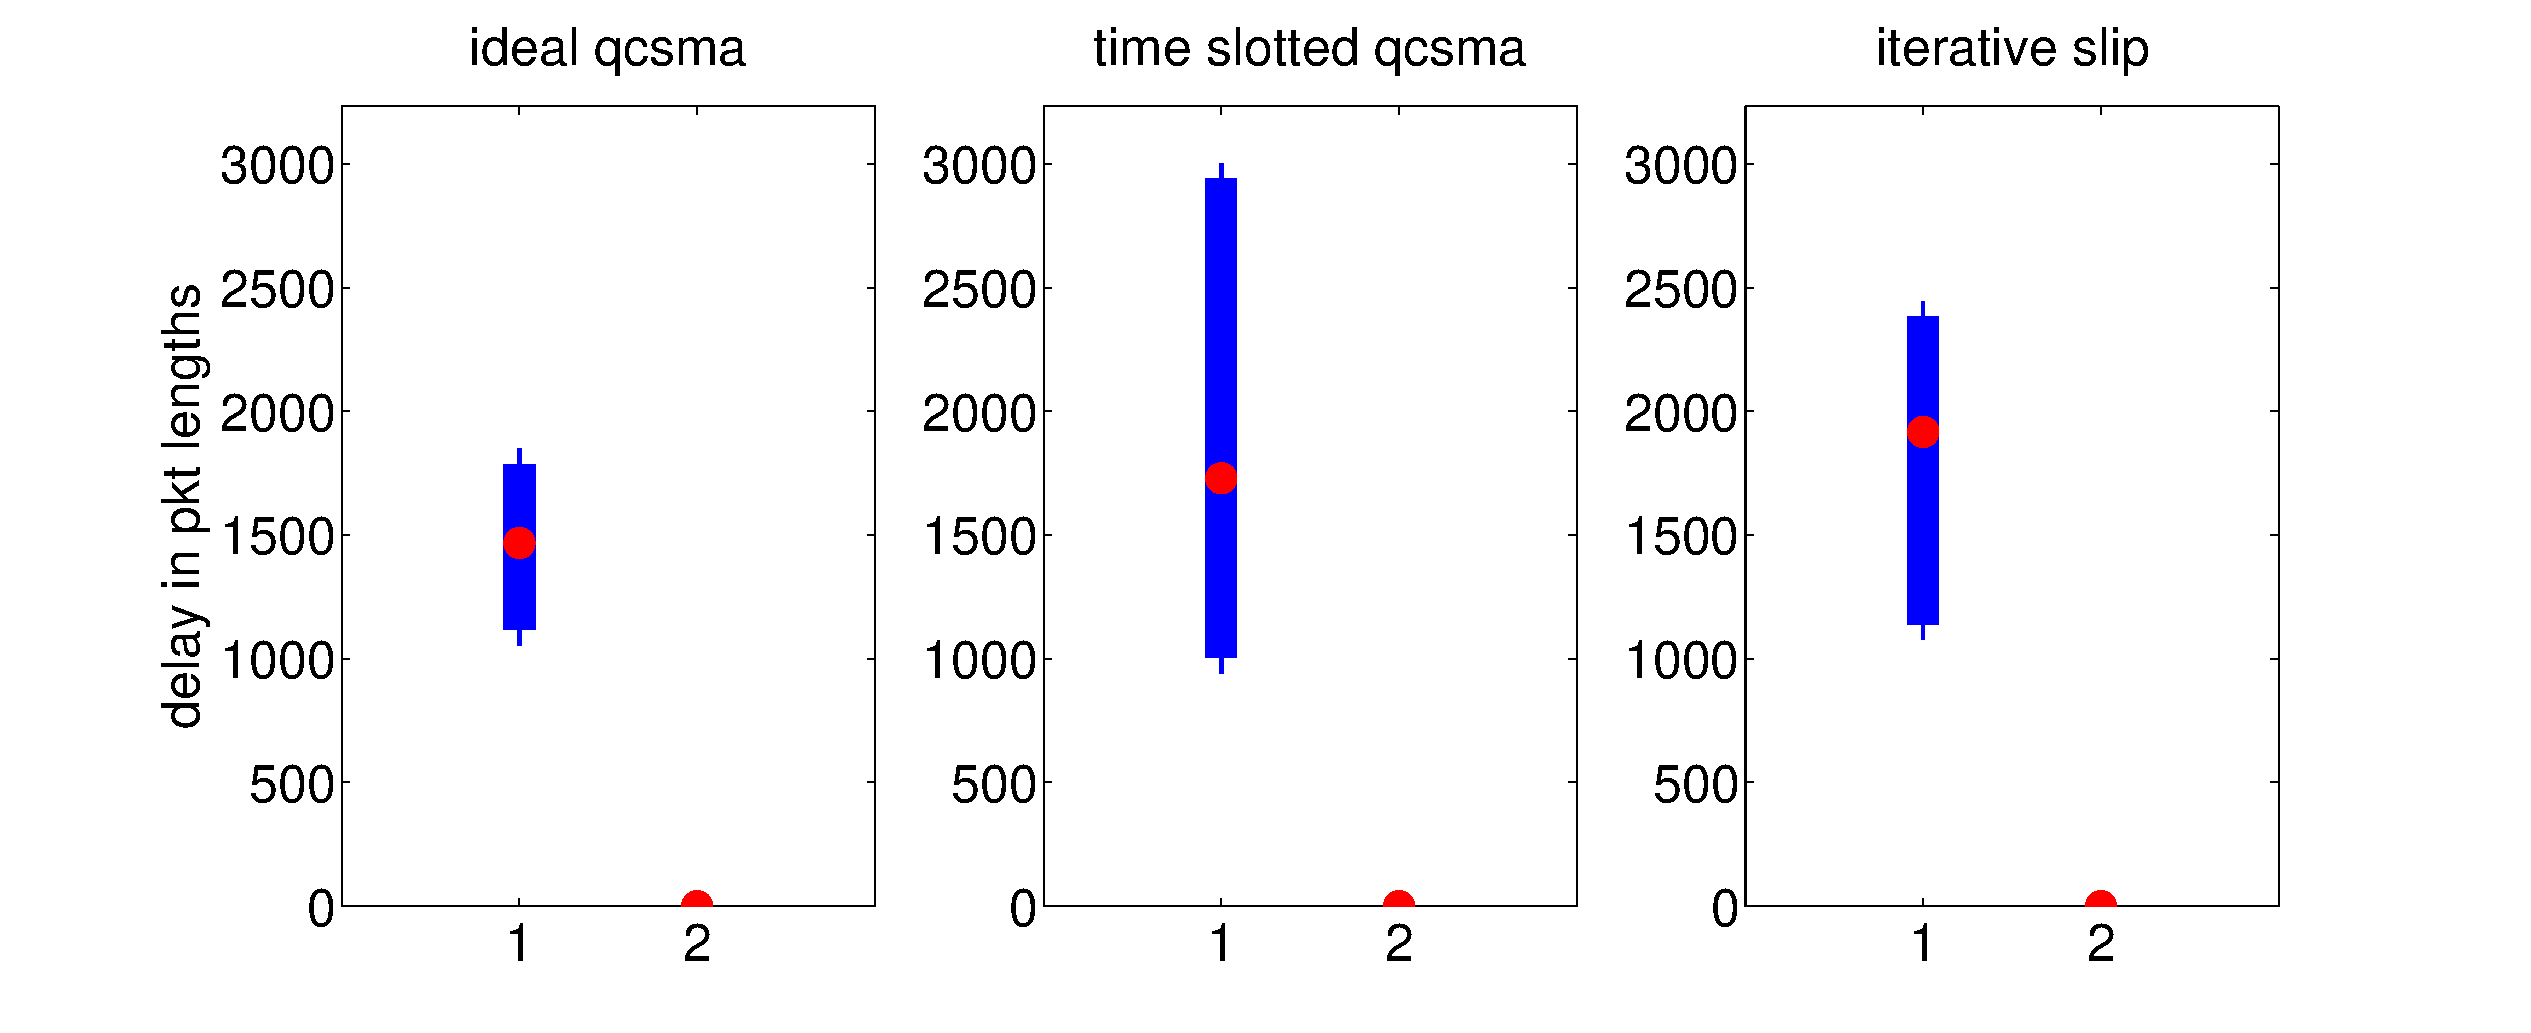
\includegraphics[width=\textwidth]{vs_spread.eps}
	\caption{This graph shows the delay spread of type 1 flows under a simulated spread and aggregate pattern.  Note the difference in average performance (as represented by the red dot).}
	\label{vs_spreadagg}
\end{figure}


\begin{figure}
\center
	 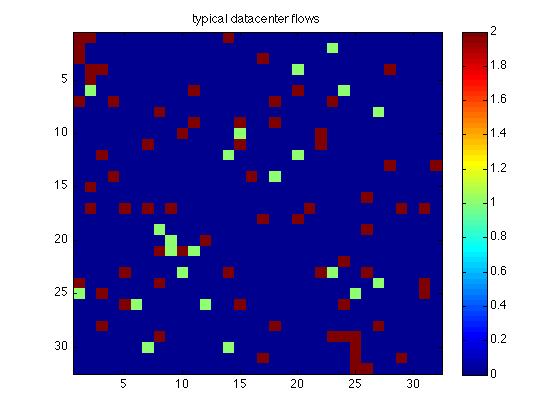
\includegraphics[width=90mm]{typ_vs_flows.png}
	\caption{This graph represents the flow matrix of a `typical' datacenter load.  Where $80\%$ of the flows (type 2) generate a low volume of traffic and are sensitive to delays.  The other $20\%$ of flows (type 1) generate a large volume of traffic and are require a high throughput but not necessarily low delays.  The color in the $s,d$th position signifies the type of flow going from input $s$ to output $d$.  Flows of type $0$ do not generate any packets.} 	
	\label{typical_flows}
\end{figure}


\begin{figure}
\center
	 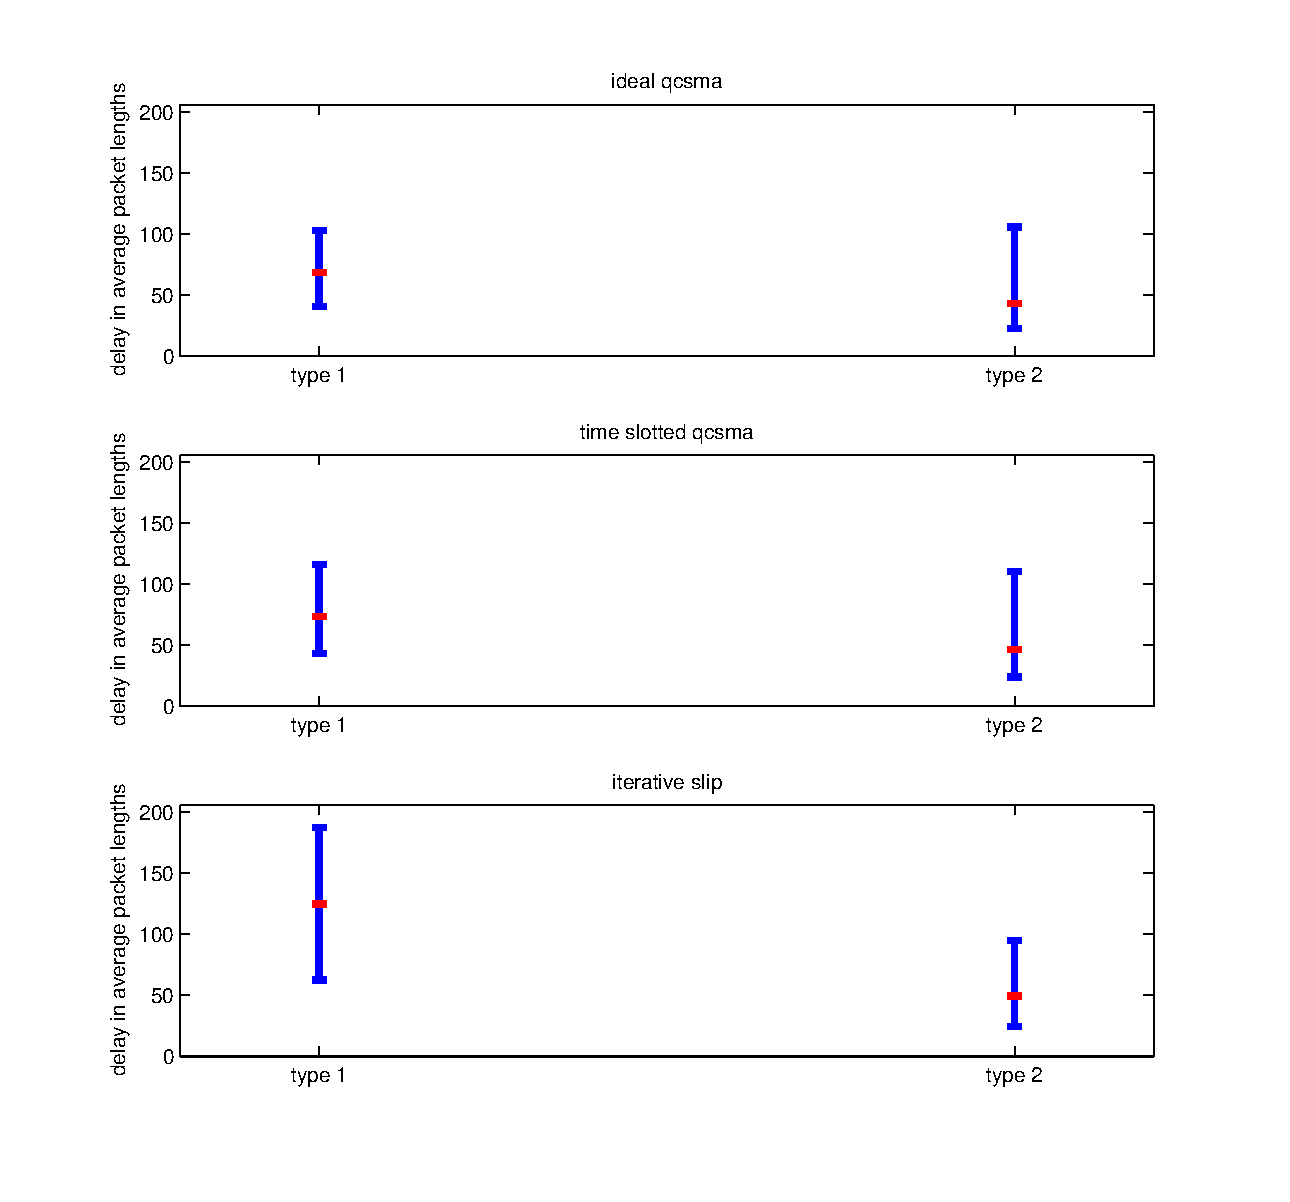
\includegraphics[width=\textwidth]{typ_vs.eps}
	\caption{This graph shows the delays experienced by a typical set of datacenter flows.}
	\label{typ_vs}
\end{figure}

\begin{figure}
\center
	 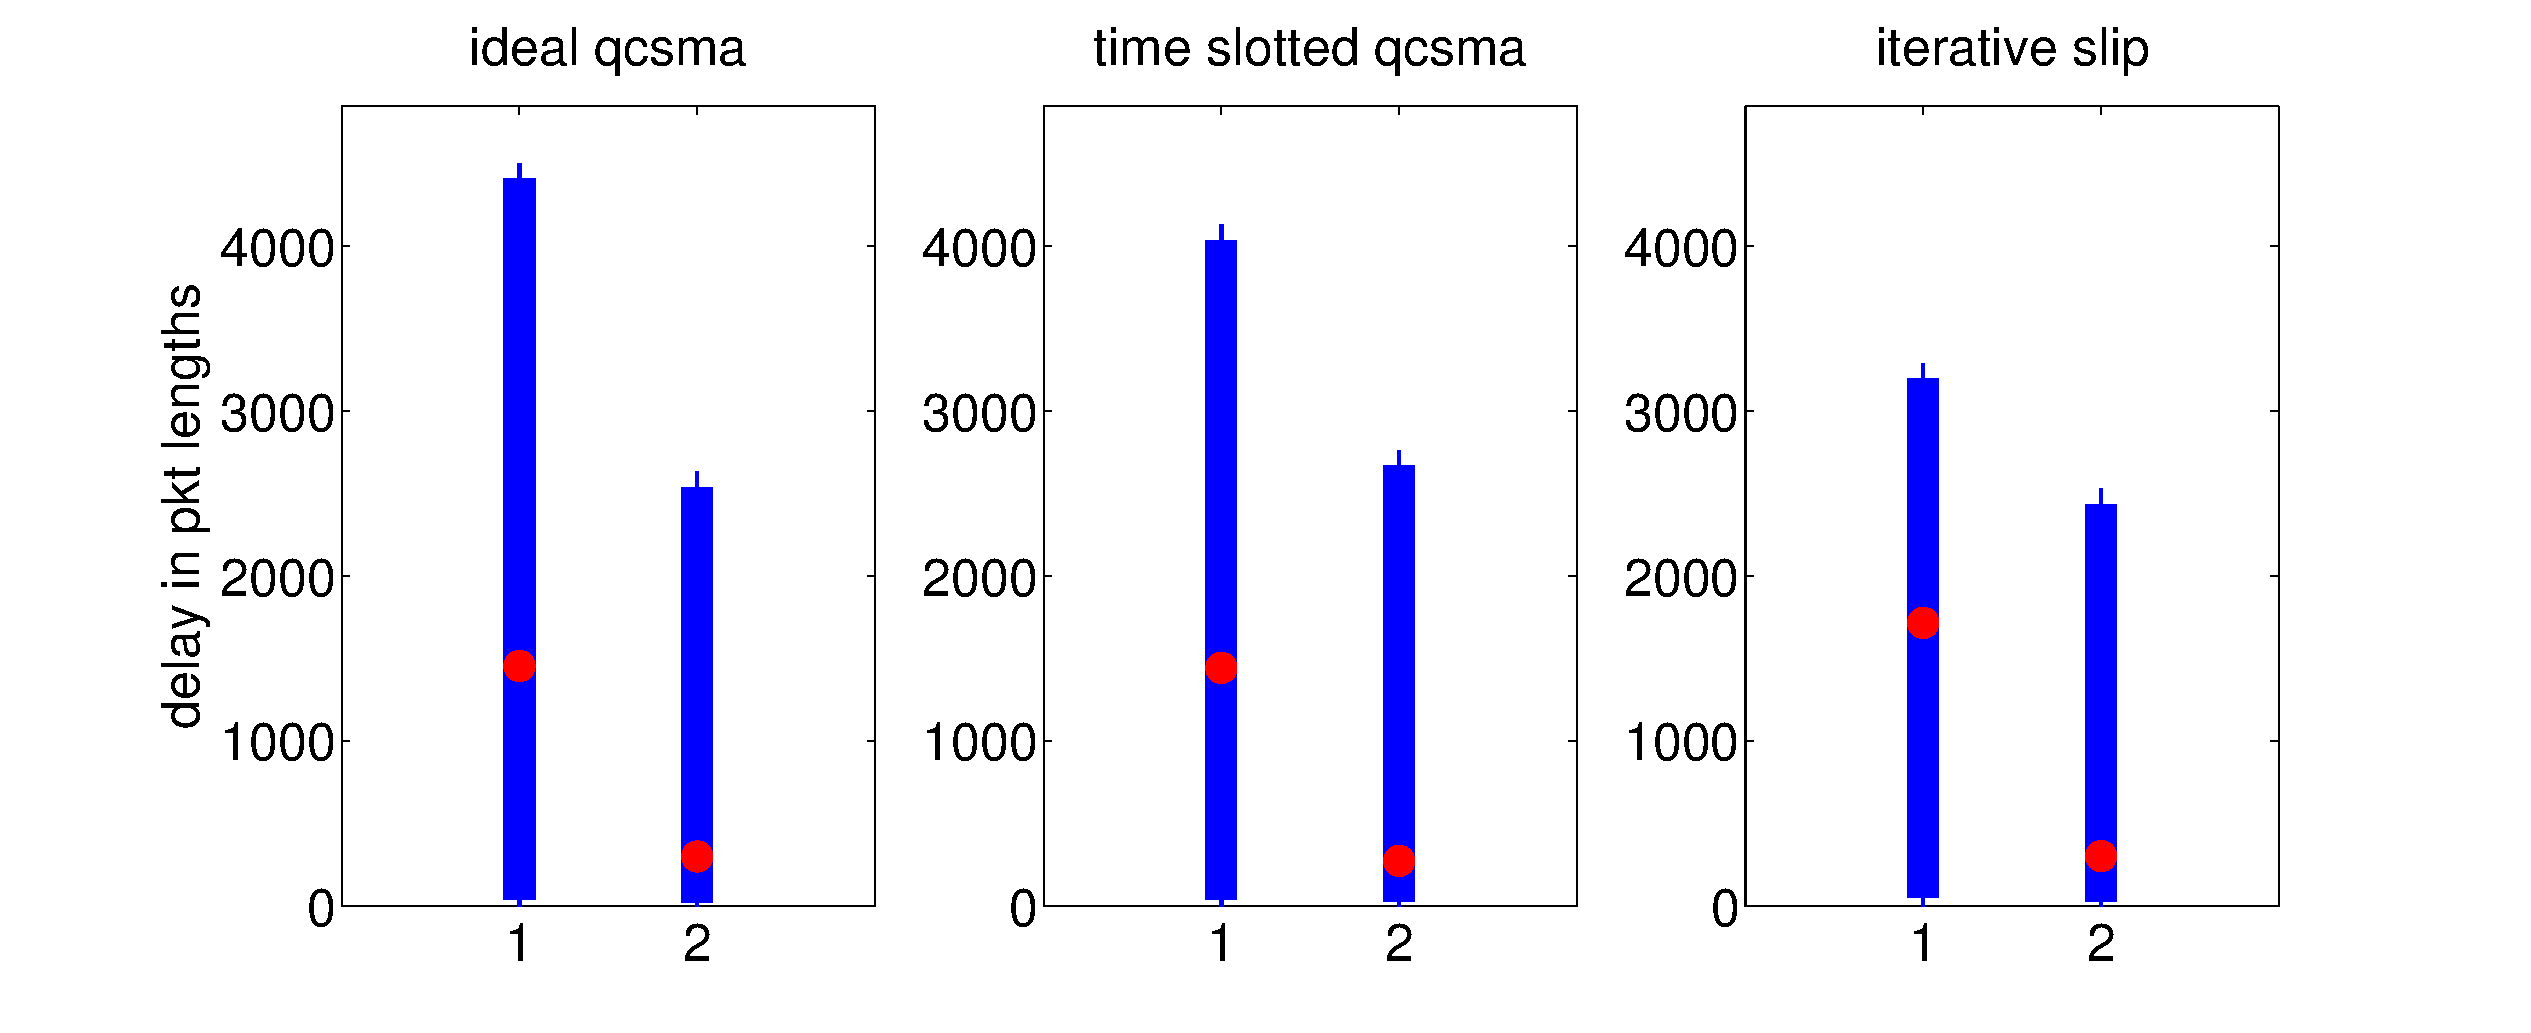
\includegraphics[width=\textwidth]{typ_spread_vs.eps}
	\caption{This graph shows the delays experienced by a typical set of datacenter flows with variable packet sizes and two spread aggregate jobs.}
	\label{typ_spread_vs}
\end{figure}


%\begin{figure}%[h]
%	 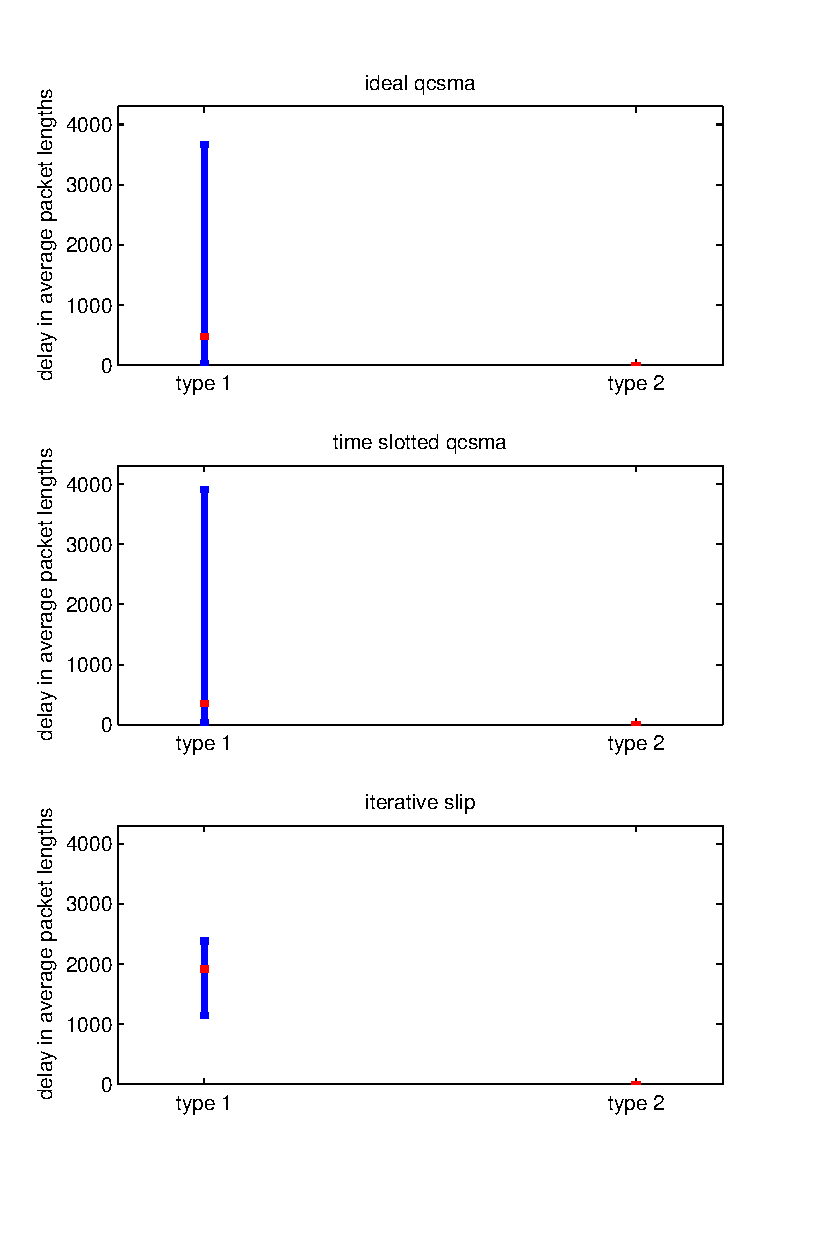
\includegraphics[width=90mm]{us_spread.eps}
%	\caption{This graph shows the delay spread of the flows under a simulated spread and aggregate pattern the packet lengths in this simulation are presumed to be equal.}
%	\label{us_spreadagg}
%\end{figure}

\subsubsection{`Typical' datacenter flows}
The statistics in \cite{Benson} and \cite{Kandula} suggest that it is normal to have a relatively low utilization of the networks in modern datacenters.  In their findings they observed that only $10\%$ of the servers communicate.  They observed that $80\%$ of the flows had very short durations, while $20\%$ flows were really long lived and responsible for the majority of transmitted bits.  To model the bimodal behavior they observed we choose to use the two types of flows mentioned above.  A sample corresponding flow pattern for our simulations can be seen in figure \ref{typical_flows}.


In our simulations for this scenario (see figure \ref{typ_vs}) QCSMA on average performs better than SLIP as usual, but also in the extremes.  The overall delays are also much less than in the other scenarios (an order of magnitude less in fact).  This is most likely due to the lower rate of competition between flows in this scenario.  This is one of the best flow patterns for both the time slotted QCSMA, which can be seen by the fact that it almost matches the performance of it's unimplementable ideal version.

%
%\begin{figure}%[h]
%	% \includegraphics[width=90mm]{typ_delays.eps}
%	\caption{This graph represents the performance generated by a `typical' datacenter load with $80\%$ low throughput delay sensitive flows (type 2) and $20\%$ high throughput delay insensitive flows (type 1).}
%	\label{typ_delays}
%\end{figure}

\subsubsection{`Typical' Flows and spread and aggregate}
Finally to explore switch performance in a datacenter setting that supports both  `typical' datacenter loads and some MapReduce like jobs, we subjected the switch to a superposition of the datacenter load and two spread and aggregate loads on servers 2 and 9 as seen in figure \ref{typ_spread_flows}.  The performance of the crossbar based switches is again comparable (see figure \ref{typ_spread_vs}).

%As can be seen in figure \ref{mixed_delay_matrix} 
The long delays seen here are due to the spread and aggregate flows for all the switches.  Note that since it is the spread and aggregate flows (all type 1 flows) that suffer, figure \ref{typ_spread_vs} shows type 1 as being particularly slow.  This is only true because the spread and aggregate flows are heavily delayed as opposed to the spread and aggregate flows slowing down other type 1 flows.  While there are some extreme outliers of type 2, the average performance is comparable to the typical data center performance.

As was to be expected, SLIP once again performed slightly worse, but not significantly.
\begin{figure}%[h]
\center
	 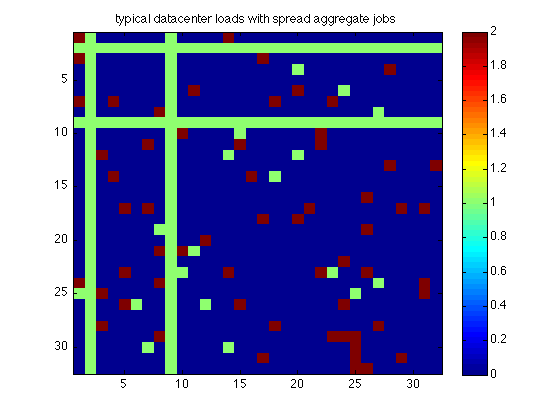
\includegraphics[width=90mm]{typ_spread_flows.png}
	\caption{This graph represents the mix of a `typical' load and two spread and aggregate jobs.}
	\label{typ_spread_flows}
\end{figure}

%\begin{figure}%[h]
%%	 \includegraphics[width=90mm]{mult2_flow_delays.eps}
%	\caption{This graph represents the performance under a mix of spread and aggregate (on servers 1 and 11) and typical flows.}
%	\label{typ_mult2_delays}
%\end{figure}
%
%\begin{figure}%[h]
%%	 \includegraphics[width=90mm]{mult2_delay_matrix.png}
%	\caption{This graph shows the average delay per flow for the mix of `typical' and spread and aggregate inputs.  The inputs originating the spread and aggregate flows (1 and 11) face the largest delays in the crossbar graphs, and here finally the ideal QCSMA differentiates itself from SLIP, but the practical QCSMA performance still remains comparable to SLIP.}
%	\label{mixed_delay_matrix}
%\end{figure}


\section{Conclusions}

Our open loop experiments (\S\ref{open}) confirmed our intuition that there is something to be gained from using the provably optimal QCSMA scheduling algorithm over iterative SLIP, although this effect has the most pronounced effect under highly loaded open loop control scenarios.  The open loop simulations also underscored the need for bookkeeping the length of the packets, as opposed to simulating a simpler scenario with equal length packets.  This is because the QCSMA algorithm works best when fewer inputs are competing for the available outputs, which is aided by a large variation in packets lengths.

In contrast, the closed loop simulations (\S \ref{closed}) we considered suggest that although there is a differentiation of performance between QCSMA and SLIP, it does not seem to play a large role in many common practical scenarios.  This is partly because the congestion levels (i.e. the loads) are adequately regulated using TCP or a similar congestion control mechanism, and partly because of the low level of intercommunication loads observed in real datacenters.

While in many scenarios the choice of scheduler seems to have a negligible effect, there is one key loading regime in which there is a significant gain from using QCSMA.  The open loop simulations correspond more closely to core and bottleneck switches, which receive lots of traffic from a large number of short-lived TCP connections.  In this scenario the tcp regulation will not have as large an impact since short-lived connections will close before their flow patterns can be significantly altered, lending a more open loop flavor to the packets flows.  For switches expected to operate in this loading regime there is much to be gained by choosing QCSMA over SLIP as a scheduling algorithm.


%% \begin{itemize}
%%\item Metric is Delay (makes sense in DataCenter Environments)
%%\item Delay VS Throughput result changes dramatically depending on packet size assumptions
%%\item TCP acts as expected
%%\end{itemize}
%%
%%\begin{itemize}
%%\item Routers are a core piece of our networks
%%\item Need simple scheduling policies, since volume of traffic strongly penalizes per packet overheads 
%%\item In the internet throughput is right metric -- can't make up for other delays in network
%%\item In Data centers have enough control over other switches that delay becomes a good metric.
%%\item Evolution of Routers -- SLIP killed head of Line delays but can't really be analyzed
%%\item QCSMA -- solves NP hard problem, but may cause large delays?
%%\item Question:  Should the optimality of QCSMA not show up in some performance gains over SLIP?  (In particular wrt delay?)
%%\end{itemize}
%%
%%\section{Schedulers}
%%\begin{itemize}
%%\item How they work
%%\item Design Philosophy
%%\item Expected Properties
%%\end{itemize}
%%
%%\section{Experiments}
%%\begin{itemize}
%%\item Uniform Packet Sizes VS More Realistic Setting
%%\item Parameter Choices
%%\item Load Graphs
%%\item TCP Graphs Choice of Load Patterns
%%\end{itemize}
%%
%%\section{Conclusions}
%%\begin{itemize}
%%\item Differences in Packet Sizes Cannot be Neglected
%%\item QCSMA may perform better than SLIP when looking at delay optimization
%%\item TCP in datacenters...
%%\end{itemize}
%%
%%\section{About Simulator:}
%%\begin{itemize}
%%\item Event Driven
%%\item variable collections
%%\item have state, events, and update functions
%%\item use memoryless thing
%%\item main loop
%%\item to change things need to change event merge, possibly the state, and which functions are called
%%\item event pictures
%%\end{itemize}
%%
%%\section{Next Step:}
%%\begin{itemize}
%%\item pick suitable parameters
%%\item Build Experiments?
%%\end{itemize}
%%\section{To Do}
%%\begin{itemize}
%%\item Build Simulator: Now -- Oct 15th?
%%\item Perform Experiments: Oct 15th -- November 15th?
%%\item Write Paper: Now -- December 15th?
%%\item Time Line
%%\end{itemize}
%%
%%\section{Simulator Pieces:}
%%\subsection{Crossbar}
%%\subsection{Scheduling Modules}
%%\subsection{Input Interface}
%%\subsection{Packet Generation}
%%\subsubsection{TCP Layer}
%%\subsubsection{Application Layer}
%%\subsection{Experiment Functions}
%%\subsection{Analysis Tools}
%%\subsubsection{Logs}
%%\subsubsection{Data Collection}
%%\subsubsection{Unit Tests}
%%\begin{itemize}
%%\item state is properly initialized
%%\item event merging
%%\item only real schedules are generated
%%\item right averages are attained
%%\item TCP waveforms are right when the channel is predictable
%%\item Event merge.
%%\end{itemize}
%%\subsubsection{Matlab Data Display Tools}
%%\subsection{Setting Parameters}
%%
%%
%%\section{Perform Experiments}
%%
%%Try to mirror the experiments with the previous simulator as much as possible.
%%\subsection{What kind of packet distributions?}
%%Try bimodal distribution with high probability around a big size and small size with slight variations around the means.  Also single size with some slight variations.  Finally try without any of the small variations.
%%\subsection{What kind of Flow patterns?}
%%Start with those we have decided model the datacenter.
%%\subsection{Throughput Vs Delay Graphs}
%%\subsubsection{What are good parameters for QCSMA?}
%%\subsubsection{Number of Slots for SLIP}
%%\subsection{TCP performance}
%%\subsection{Performance Variation as packet sizes become more predictable}
%%
%%\section{Write Paper}
%%\subsection{Would like to show: QCSMA is better than SLIP by x\%}
%%\subsection{Would like to show: Equal Length vs Variable Length Packets makes a big difference!}
%%\subsection{Simulator Documentation}
%%\subsubsection{Events and State}
%%\subsubsection{How to change things}
%%

\label{bib}
\bibliography{MSThesis}{}
\bibliographystyle{plain} 
 \newpage
\appendix
%  \appendices 
 \section{Simulator Design} \label{code_design}
 
 Because the simulation tracked events on two very different time scales (that of packet transmissions and that of schedulers clock ticks) we chose to use an event driven simulator.  This means that we had a mechanism for calculating the next event (and time at which it occurred) given the current state of the system, instead of calculating the new state at each time step.
 
 \subsection{Main components} \label{maincomp}
 To accommodate this simulation model, the heart of the code was split into essentially two logical pieces: State variables, and state transitions.  Logically, the heart of the simulator looks like this:
 \begin{verbatim}
 while(num_events<tot_num_events)
 {
      event = next_event()
      update_state(event)
      num_events=num_events+1
 }
 \end{verbatim}
 The update$\_$state() function, takes a state transition (in the form of an instantiation of the Event class) and calculates the new state of the system.  Similarly, the next$\_$event() function calculates the next state transition based on the current state of the system.  Of course there are sanity checks built in, machinery to setup the initial state, and machinery used to record the results of the calculation, but at the most basal level, this is what the simulator is doing.  To understand this function I will talk briefly about what constitutes the state, what an event is, and how the next event is calculated.
 
 \subsubsection{State}
 
The state with a few minor exceptions mainly of different queues of packets which contain the crucial information about where to route the packets and when they arrived into the system.  Generally each state is regulated by a particular kind of event.
\begin{itemize}
\item {\bf Current Time}\\
 --  This variable determined the time elapsed in scheduler clock ticks since the start of the simulation.
\item {\bf Packet Generation State}\\
 --  For the simulations which generated packets as Markov chains as inputs each flow had an associated state (ON or OFF)
\item {\bf Flow Queues}\\
 --  Upon generation each packets are placed in flow queues, which represent queues of different application flows within a computer.  Depending on the simulation, packets would stay in here until released by the TCP flow regulator.
\item {\bf NIC state}\\
 --  This state keeps track of which flows are being transferred from the ``computer" and transferred to the network.  In the closed loop simulations this is regulated by the TCP state.
\item {\bf Switch Queues}\\
--  Once a packet is transferred out of the flow queues, it is placed into the switch queues, which in conjunction with the crossbar state is used to calculate the next scheduler events.
\item {\bf Crossbar State}\\
--  The crossbar state keeps track of which inputs and outputs are currently transmitting packets and how much longer it will take to finish the transmission.
\item {\bf Event Heap (ACKs)}\\
--  Upon exit of the system, and ACK along with an appropriate arrival time is generated and placed onto the event heap.  
\end{itemize}

\subsubsection{Events}

All changes to the state occur through the application of an Event object to the state through the update$\_$state() function.  So essentially, an Event object consists of three things: the change to be applied to the state, the time at which it occurs, and a merge() function, to calculate a new Event from two candidate Events.  Of these three things, the merge() is the only one which is the least straightforward:
\begin{verbatim}
Event merge(event)
{
     if(event occurs before this)
     {
          return event
     }
     if(event occurs after this)
     {
           return this
     }
     if(event occurs simultaneously with this)
     {
            include both state changes
            return this
     }
}
\end{verbatim}

Given this structure the next$\_$event() function is philosophically structured as follows:

\begin{verbatim}
Event next_event()
{
     event = next_pkt_gen()
     event.merge(next_nic_update())
     event.merge(next_crossbar_update())
     event.merge(event_heap.next_ack())
     return event
}
\end{verbatim}

Notice that there is no effort to save the events that the merge() function discards.  This is because the stochastic events are generated in a memoryless fashion parametrized by the state (i.e. either occur or do not with the same probability at each time step).  The deterministic events are all a function of the state and can be recalculated from the new state that results after the application of an earlier event.  The ACKs are stored in the event$\_$heap, but could in theory also have their own state variable.  Other deterministic events could also be stored in the event$\_$heap depending on the preference of the coder.

So to add a component of a simulator it would be necessary to do the following things:
\begin{itemize}
\item Create additional state variable\\
--- This is to facilitate any bookeeping necessary for events generated by this new component
\item Update the Event class to include updates to the new state.\\
--- This consists of two important parts: a modification of variables in the Event class, and an update to the {\it merge()} function, so two events modifying your new state can successfully be merged into one.
\item The creation of a new function to be placed into the next$\_$event() function.\\
--- This new function would have the form of a next$\_${\it new$\_$component}$\_$event() and would calculate the next event that would occur given the current state.
\item Ideally there would also be a control variable allowing for an easy way to remove the component if it is not needed in a simulation.
\end{itemize}
%%
%%\begin{itemize}
%%\item To illustrate what the functions called by next$\_$event() look like we have the example of:
%%\item To add a component to the simulator, need to modify:
%%\item switch statements 
%%\end{itemize}
\subsection{Auxiliary structures}
In addition to the simulation mechanisms there are a few code structures meant to improve the ease of use.  Data is collected by entering it into an object of the Data$\_$Collector class which provides a convenient dump$\_$to$\_$file() function, which dumps the data into a csv file.  Once all the data is recorded in a file, you can easily graph the data using a Matlab script.\\

Because of the size of the simulator, there are many sets of variables floating around which may make it difficult to follow what is relevant to what.  In order to combat this, the simulator has collected the different variables parametrizing the different components in structs such as the TCP$\_$State or the Scheduler$\_$Parameters struct, defined at the beginning of the code so that it is easy to follow what values need to be defined in order to make the simulator function.\\

Another issue with understanding the simulator code is that it contains components that can be added or removed (such as the TCP layer or the current choice of scheduler).  What simulator components are currently active is parametrized by the Simulation$\_$Parameters struct, and at the relevant places in the code, there is a switch statement or a an if statement which switches between the relevant components.  Searching for the variables collected in Simulation\_Parameters should quickly reveal any places that have been modified or need to modified by the particular component.
%%\begin{itemize}
%%\item variable collections and switch statements
%%\item Data Collector Class
%%\item Matlab
%%\end{itemize}

\subsection{Function Descriptions}
\subsubsection{Data\_Collector}
This class was designed to make data collection intuitive and easy.  Essentially when you initialize a data collector object you can index the type of statistic you would like to collect and add labels and types of data.  Then at the appropriate parts of the code you can easily add the value to the appropriate statistic.  Finally the Data Collector comes with a convenient dump to file function which allows the statistics collected be written to a csv file which is easy to load into a Matlab script.
\begin{itemize}
\item {\bf Initialization:}\\
To initialize a data collection object, call its constructor with the number of statistics types to be collected.  The function for specifying a specific stat is a little more complicated:
\begin{verbatim}
	initialize_stat(int stat_index,string name,int type,
	                      int num_rows,int num_cols,bool user_defines_count)
\end{verbatim}
This functions allows you to specify the index by which to call the stat, specify a name, a type (average, max, or variance), the number of rows and columns that the stat will have, and whether or not the user will specify the divisor for dumping to a file.  If the count is not specified by the user, the data collected (if it is not a max) is divided by the number of data added.
\item {\bf Record}\\
Once the stats have been initialized a new piece of data can be added easily using the function:
\begin{verbatim}
       enter_data(int stat_index,int stat_row,int stat_col,int new_data)
\end{verbatim}
Where all you need to specify is the index of the stat to be modified, and which row and column is affected as well as the new piece of data to be recorded.  If the count is specified by the user as the final time of the simulation you often want to multiply the relevant data by the time elapsed since the last time the data was recorded.
\item {\bf Output}\\
Printing the data to an output file uses the function:
\begin{verbatim}
        dump_to_file(string file_name,int specified_count)
\end{verbatim}
  In this case the specified\_count is applied to all the statistics which had the user\_defines\_count flag set to true.  The output is then printed in the format of having each stat printed consecutively:
  \begin{verbatim}
        row, col
        stat[0][0],stat[0][1],stat[0][2],....stat[0][col-1]
        .
        .
        .
        stat[row-1][0] ,..., stat[row-1][col-1]
\end{verbatim}
followed by the next stat.
\end{itemize}

\subsubsection{Control and State Variables}
The simulation state and control variables are contained in the following structs:
\begin{itemize}
\item Slip\_State slip\_state
\item TCP\_State tcp\_state
\item Scheduler\_Parameters sched\_par
\item Simulation\_Parameters sim\_par
%\item flow variables\item switch statements
\end{itemize}
The variables contained in these structs are mostly self explanatory.  If they are not a part of an active state, but rather a parameter the variables are limited to being used to activate `switch' statements or `if' statements at the appropriate places in the code, so understanding their effects should be relatively simple.

\subsubsection{Simulation Functions}
Different simulations can now be run by changing the appropriate parameters and resetting the state to zero.  The basic functions for doing this are the following:
\begin{itemize}
\item init\_sim\\
Sets all the initial parameters including the hardwired choice of scheduler parameters.
\item reset\_sim\\
Leaves all the parameters alone but resets the state.  (e.g. empties the event queues, and flushes any packets from the system.)
\item run\_sim\\
This function runs the simulation forward for the specified number of events using the set of parameters set by other functions.  In particular enters the `while' loop described in \ref{maincomp}.
\item tcp\_load\_sim\\
Uses a combination of init\_sim and reset\_sim as well as some more specialized flow patterns and specific adjustments to parameters to run the tcp simulations.
\item iid\_load\_sim\\
Similar to tcp\_load\_sim this function runs the open loop tests.
\end{itemize}


\subsubsection{Event Sim Mechanics}
These functions are needed to update the various states and handle events properly:
\begin{itemize}
\item update\_state\\
See \ref{maincomp}.
\item next\_event\\
Also see \ref{maincomp}.
\item geo\_exp\\
This function generates an outcome corresponding to the first expirations of a set of geometric random variables.  Many of the other functions are built on this.
\end{itemize}

\subsubsection{Flow patterns}
This is just the set of functions that generate the different flow patterns with the exception of separate dump\_flows\_to\_file which allows you to easily print out the flows to a csv file in a similar format to the Data\_Collector object:
\begin{itemize}
\item dump\_flows\_to\_file
\item dc\_flow\_pattern
\item spread\_pattern
\item all\_2\_all\_pattern
\end{itemize}

\subsubsection{Scheduler Machinery}
Of course the heart of the scheduler needs to simulate the scheduling algorithms:
\begin{itemize}
\item idle\_c\_bar
\item basic\_slotted\_qcsma
\item islip
\item pkt\_to\_cells\\
A helper function to break large packets into smaller packets when slip is used.
\end{itemize}

\subsubsection{TCP Functions}
Finally TCP has a collection of helper functions to properly update the state when TCP is being used: 
\begin{itemize}
\item tcp\_update\\
Update the tcp\_state struct, which keeps track of the TCP window, the packets sent, round trip time estimates etc.
\item should\_tcp\_send\\
Determines whether the packet should be sent to the switch base on the TCP window and the currently sent packets.
\item gen\_ack\\
Generates an ack and places it on the event queue whenever a packet exits the system.
\end{itemize}






\end{document}